% 第 5 章 双坐标与转移映射
% 来源：docs/paper-submission/main.tex §"The separation is a transition-map invariant"
%       （Lemma realT、eq. taun、Thm welding、Cor. cn）、Remark invariance；
%       docs/paper-submission/sec-general.tex Prop. gen-base、Cor. gen-invariant。
% 数值：figures/ch05_transition_example.py（调用 docs/transition_map.py）；图：figures/fig5_cylinders.py。

\chapter{双坐标与转移映射}\label{ch:transition}

设 $(f_s,w_0)$ 是一个实鞍结开折（\cref{def:unfolding}），$s>0$ 固定。
本书关心的``分数次迭代''是 Abel 型函数方程
\begin{equation}\label{ch5:eq:abel}
 K(z+1)=f_s\bigl(K(z)\bigr),\qquad K(0)=w_0
\end{equation}
的全纯解。这样的解有无穷多个。其中两个是经典的：吸引不动点 $L$ 处的正则解 $R$
和排斥不动点 $L_2$ 处的正则解 $S$（第~\ref{ch:koenigs} 章）。它们各自只在``一半''的复平面上有好的性质：
$R$ 在虚方向有周期 $\ii h$，$S$ 有周期 $\ii h_2$，两个周期不同，所以没有一个解能同时等于两者。

本章的主角是两个正则解之间的\textbf{转移映射}
\[
 T=R^{-1}\circ S .
\]
它是一个``平移加周期函数''，只依赖于映射 $f_s$ 和基点，而与``选哪个分数次迭代''无关。
本章证明两件事。第一，$T$ 的 Fourier 系数经过规范化之后（$\tau_n$），其模长与基点无关，
并且在实解析共轭下不变。第二（焊接恒等式），任何一个上方用 $R$ 表示、下方用 $S$ 表示的解 $K$，
它偏离 $R$ 的系数 $c_n$ 与 $T$ 的系数之间有一个精确的恒等式。因此``分离''是映射的不变量，
不是某个构造方法的产物。第~\ref{ch:sewing} 章再用这个恒等式构造并刻画缝合解。

\begin{goals}
\item 两个正则解 $R$、$S$ 及其实结构；转移映射 $T=R^{-1}\circ S$，它的 Fourier 系数 $t_n$ 与不变量 $\tau_n=t_n\ee^{-2\pi\ii nt_0}$。
\item 实结构引理：实轴上 $\Ima T\equiv h/2\pmod h$；取 $\Ima t_0=h/2$ 的分支。由此 $|t_n|=|\tau_n|\Lam^{n/2}$。
\item 换基点只让 $\tau_n$ 乘上 $\ee^{2\pi\ii n\Delta}$（$\Delta$ 实）；所以 $|\tau_n|$、$|B_n|$、$\Rea\kappa^{(n)}_j$ 是开折在保持定向的实解析共轭下的不变量。
\item 双侧解的分离系数 $c_n$，平移规范，规范无关比值 $\Xi_n=c_n/c_1^n$。
\item 焊接恒等式 $t_n=\sum_{m\ge n}c_m[\ee^{2\pi\ii mG}]_{n-m}$，以及``缝口在实轴下方半个周期''如何产生尺度 $\Lam^n$。
\end{goals}

本章固定一个实鞍结开折 $(f_s,w_0)$，满足 (H1)--(H4)；(H5) 不用。$s\in(0,s_2]$ 取第~\ref{ch:unfolding} 章实动力学引理中的范围，
并在不致混淆时省略下标 $s$，写 $f=f_s$。沿用第~\ref{ch:unfolding} 章的记号：
$L<L_2$ 是两个实不动点，乘子 $0<\lambda_1<1<\lambda_2$，
\[
 h=\frac{2\pi}{|\log\lambda_1|},\qquad h_2=\frac{2\pi}{\log\lambda_2},\qquad \Lam=\ee^{-2\pi h}.
\]

% ======================================================================
\section{两个正则解}\label{ch5:sec:RS}

记 $\mathcal A(L)$ 为 $L$ 的吸引域。设 $\sigma$ 是 $L$ 处的 Koenigs 坐标，
$\sigma\circ f=\lambda_1\sigma$，$\sigma'(L)=1$，并按 $\sigma=\lambda_1^{-n}\,\sigma\circ f^n$ 延拓到整个 $\mathcal A(L)$
（\cref{thm:koenigs}）。设 $\sigma_{\rm rep}$ 是 $L_2$ 处的 Koenigs 坐标，
$\sigma_{\rm rep}\circ f=\lambda_2\sigma_{\rm rep}$，$\sigma_{\rm rep}'(L_2)=1$。它的逆 $\sigma_{\rm rep}^{-1}$ 在 $0$ 附近有定义，
并由
\[
 \sigma_{\rm rep}^{-1}(\zeta)=f^n\bigl(\sigma_{\rm rep}^{-1}(\zeta/\lambda_2^n)\bigr)
\]
延拓为整函数（$f$ 是整函数，(H1)）。这是 Poincaré 函数的经典构造。

\begin{definition}[两个正则解]\label{ch5:def:RS}
\begin{enumerate}
\item \textbf{吸引正则解} $R$ 是 \cref{def:regular-solution} 中以 $w_0$ 为初值的解：$R(0)=w_0$，且
  \begin{equation}\label{ch5:eq:sigmaR}
   \sigma\bigl(R(z)\bigr)=\sigma(w_0)\,\lambda_1^{\,z}
  \end{equation}
  在 $R$ 有定义的地方成立。它的逆，即\textbf{吸引 Abel 坐标}，是多值函数
  \begin{equation}\label{ch5:eq:Rinv}
   R^{-1}(w)=\frac{\log\bigl(\sigma(w)/\sigma(w_0)\bigr)}{\log\lambda_1},\qquad w\in\mathcal A(L),\ \sigma(w)\ne0 .
  \end{equation}
\item \textbf{排斥正则解}是整函数
  \begin{equation}\label{ch5:eq:S}
   S(z):=\sigma_{\rm rep}^{-1}\bigl(-\lambda_2^{\,z}\bigr).
  \end{equation}
\end{enumerate}
\end{definition}

\begin{lemma}[两个正则解的基本性质]\label{ch5:lem:RS}
\begin{enumerate}
\item $R(z+1)=f(R(z))$，$R(z+\ii h)=R(z)$；$R^{-1}$ 的任意两个分支相差 $\ii h\Z$ 中的常数，并且
  对 $R$ 有定义的每个 $z$，$R^{-1}(R(z))\in z+\ii h\Z$。
\item $S(z+1)=f(S(z))$，$S(z+\ii h_2)=S(z)$。
\item $S$ 把 $\R$ 严格递减地映满 $(L,L_2)$：$S(x)\to L_2$（$x\to-\infty$），$S(x)\to L$（$x\to+\infty$），并且 $S'(x)<0$。
\item 在 $(L,L_2)$ 上 $\sigma>0$、$\sigma'>0$；而 $\sigma(w_0)<0$。
\end{enumerate}
\end{lemma}

\begin{proof}
(1) 函数方程由 \eqref{ch5:eq:sigmaR} 与 $\sigma\circ f=\lambda_1\sigma$ 得到；周期性来自
$\lambda_1^{\ii h}=\ee^{\ii h\log\lambda_1}=\ee^{-2\pi\ii}=1$。$\log$ 的分支相差 $2\pi\ii k$，
除以 $\log\lambda_1=-2\pi/h$ 得 $-\ii hk$。由 \eqref{ch5:eq:sigmaR}，$\sigma(R(z))/\sigma(w_0)=\lambda_1^z=\ee^{z\log\lambda_1}$，
所以 $\log(\sigma(R(z))/\sigma(w_0))\in z\log\lambda_1+2\pi\ii\Z$，即 $R^{-1}(R(z))\in z+\ii h\Z$。

(2) $S(z+1)=\sigma_{\rm rep}^{-1}(\lambda_2\cdot(-\lambda_2^z))=f(S(z))$；周期性同 (1)。

(3) 由 第~\ref{ch:unfolding} 章实动力学引理的 (3)，$f$ 在 $[L,L_2]$ 上递增，把 $(L,L_2)$ 映入自身，其中的轨道递减地趋于 $L$。
在 $0$ 的一个小邻域里，$\sigma_{\rm rep}^{-1}$ 在负实轴上取 $(L,L_2)$ 中的实值且递增。
对 $t>0$ 任意，取 $n$ 使 $t/\lambda_2^n$ 足够小，则 $\sigma_{\rm rep}^{-1}(-t)=f^n(\sigma_{\rm rep}^{-1}(-t/\lambda_2^n))\in(L,L_2)$，
并且（链式法则，$f'>0$ 在 $[L,L_2]$ 上）$\frac{\dd}{\dd t}\sigma_{\rm rep}^{-1}(-t)<0$。由于 $-\lambda_2^x$ 随 $x$ 递减，
$S'(x)=(\sigma_{\rm rep}^{-1})'(-\lambda_2^x)\cdot(-\lambda_2^x\log\lambda_2)<0$。
$x\to-\infty$ 时 $-\lambda_2^x\to0^-$，$S(x)\to L_2$；$x\to+\infty$ 时 $S(x+n)=f^n(S(x))\to L$。

(4) $\sigma>0$ 于 $(L,L_2)$ 与 $\sigma(w_0)<0$ 是 第~\ref{ch:unfolding} 章实动力学引理的 (5)。
对 $w\in(L,L_2)$，$\sigma'(w)=\lambda_1^{-n}\sigma'(f^nw)\,(f^n)'(w)$；$n$ 大时 $f^nw$ 靠近 $L$，$\sigma'(f^nw)\approx1$，
而 $(f^n)'(w)>0$，所以 $\sigma'(w)>0$。
\end{proof}

\begin{remark}[负号的作用]\label{ch5:rem:sign}
\eqref{ch5:eq:S} 中的负号使 $S$ 的实轴落在两个不动点之间的线段 $(L,L_2)$ 上。如果用 $+\lambda_2^z$，
$S(\R)$ 是 $(L_2,\cdots)$ 一侧的逃逸轨道，不在 $L$ 的吸引域里。$S$ 在实方向的平移
（即 $\sigma_{\rm rep}^{-1}(-c\lambda_2^z)$，$c>0$）不影响本章的任何不变量（\cref{ch5:rem:normalisations}）。
\end{remark}

% ======================================================================
\section{转移映射}\label{ch5:sec:T}

\begin{lemma}[转移映射的定义域]\label{ch5:lem:strip}
存在 $\vartheta>0$，使得在水平带 $\Sigma=\{|\Ima z|<\vartheta\}$ 上 $S(z)\in\mathcal A(L)$ 且 $\sigma(S(z))\ne0$。
设 $\mathcal L(z)$ 是 $\log\bigl(\sigma(S(z))/\sigma(w_0)\bigr)$ 在 $\Sigma$ 上的一个连续分支。则
\begin{enumerate}
\item $\Ima\mathcal L$ 在实轴上是常数，并且属于 $\pi+2\pi\Z$；
\item $\mathcal L(z+1)=\mathcal L(z)+\log\lambda_1$ 对 $z\in\Sigma$ 成立。
\end{enumerate}
\end{lemma}

\begin{proof}
$S([0,1])$ 是 $(L,L_2)$ 中的紧集，$(L,L_2)\subset\mathcal A(L)$ 且其上 $\sigma>0$（\cref{ch5:lem:RS}(4)）。
$\mathcal A(L)$ 是开集，$\sigma$ 连续，所以存在 $\vartheta>0$ 使 $z\in[0,1]+\ii(-\vartheta,\vartheta)$ 时
$S(z)\in\mathcal A(L)$、$\sigma(S(z))\ne0$。对一般的 $z\in\Sigma$，写 $z=z'+n$，$z'\in[0,1]+\ii(-\vartheta,\vartheta)$，$n\in\Z$。
若 $n\ge0$，$S(z)=f^n(S(z'))$；若 $n<0$，$f^{|n|}(S(z))=S(z')$。两种情形下 $S(z)\in\mathcal A(L)$
（吸引域在 $f$ 和 $f^{-1}$ 下完全不变），且 $\sigma(S(z))=\lambda_1^{n}\sigma(S(z'))\ne0$。$\Sigma$ 单连通，所以连续分支存在。

(1) 对实的 $x$，$\sigma(S(x))>0>\sigma(w_0)$，比值为负，所以 $\Ima\mathcal L(x)\in\pi+2\pi\Z$；它连续，故为常数。

(2) $\sigma(S(z+1))=\sigma(f(S(z)))=\lambda_1\sigma(S(z))$，所以 $\mathcal L(z+1)-\mathcal L(z)-\log\lambda_1\in2\pi\ii\Z$，
由连续性是常数 $2\pi\ii k$。在实轴上取虚部，由 (1) 得 $0=0+0+2\pi k$，故 $k=0$。
\end{proof}

\begin{definition}[转移映射]\label{def:transition}
在 \cref{ch5:lem:strip} 的带 $\Sigma$ 上，令
\[
 T(z):=R^{-1}\bigl(S(z)\bigr)=\frac{\mathcal L(z)}{\log\lambda_1}.
\]
称 $T$ 为\textbf{转移映射}（transition map）。由 \cref{ch5:lem:strip}(2)，$T(z+1)=T(z)+1$，
所以 $T-\id$ 是 $\Sigma$ 上 $1$-周期的全纯函数，有 Fourier 展开
\begin{equation}\label{ch5:eq:Tfourier}
 T(z)-z=\sum_{n\in\Z}t_n\,\ee^{2\pi\ii nz},\qquad
 t_n=\int_{x_0+\ii y}^{x_0+1+\ii y}\bigl(T(z)-z\bigr)\ee^{-2\pi\ii nz}\,\dd z ,
\end{equation}
积分可以取在 $\Sigma$ 中的任何水平线段上（Cauchy 定理与周期性）。$T$ 的分支是 $T+\ii hk$（$k\in\Z$），
它们只改变 $t_0$。我们总取
\begin{equation}\label{ch5:eq:branch}
 \Ima t_0=\frac h2
\end{equation}
的那一支（\cref{lem:realT} 说明它存在且唯一），并定义
\begin{equation}\label{ch5:eq:tau}
 \tau_n:=t_n\,\ee^{-2\pi\ii nt_0}\quad(n\ge1),\qquad
 T^\circ:=T-\id-t_0=\sum_{n\ne0}t_n\ee^{2\pi\ii nz}.
\end{equation}
\end{definition}

\begin{lemma}[实结构]\label{lem:realT}
对每个实数 $x$，$\Ima T(x)\equiv h/2\pmod h$。因此存在唯一的分支使 $\Ima t_0=h/2$；在这一支上：
\begin{enumerate}
\item $\Ima T(x)=h/2$ 对所有实 $x$ 成立，即 $T(x)-x-\ii h/2$ 是实值函数；
\item $t_{-n}=\overline{t_n}$（$n\ne0$），$T^\circ$ 在实轴上取实值；
\item $T'(x)>0$，并且 $T-\ii h$ 把 $\R$ 双射地映到直线 $\{\Ima w=-h/2\}$ 上，与 $z\mapsto z+1$ 交换。
\end{enumerate}
\end{lemma}

\begin{proof}
由 \cref{ch5:lem:strip}(1)，$\Ima\mathcal L(x)=(2k+1)\pi$ 是常数。除以 $\log\lambda_1=-2\pi/h$：
\[
 \Ima T(x)=\frac{(2k+1)\pi}{\log\lambda_1}=-\Bigl(k+\frac12\Bigr)h\equiv\frac h2\pmod h .
\]
换分支 $T\mapsto T+\ii hk'$ 可以让这个常数等于 $h/2$，且只有一种取法。由于 $\Ima(T(x)-x)$ 是常数 $c$，
$\Ima t_0=\Ima\int_0^1(T(x)-x)\dd x=c$；所以 $\Ima t_0=h/2$ 与 (1) 等价。

(2) $T(x)-x-\ii h/2$ 是实值 $1$-周期函数，其 Fourier 系数满足 $\hat F_{-n}=\overline{\hat F_n}$；
它的系数就是 $t_n$（$n\ne0$）与 $t_0-\ii h/2$。$T^\circ$ 是它减去实常数 $\Rea t_0$。

(3) 在实轴上 $T(x)=\log\bigl(\sigma(S(x))/|\sigma(w_0)|\bigr)/\log\lambda_1+\ii h/2$（实对数），所以
\[
 T'(x)=\frac{\sigma'(S(x))\,S'(x)}{\sigma(S(x))\,\log\lambda_1}.
\]
由 \cref{ch5:lem:RS}(3)(4)，分子为负（$\sigma'>0$，$S'<0$），分母为负（$\sigma>0$，$\log\lambda_1<0$），故 $T'(x)>0$。
于是 $x\mapsto T(x)-\ii h=\Rea T(x)-\ii h/2$ 是 $\R$ 到 $\{\Ima w=-h/2\}$ 的严格递增映射；$T(x+1)=T(x)+1$
说明它是满射，且与平移 $1$ 交换。
\end{proof}

\begin{remark}[$\tau_n$ 依赖于什么]\label{ch5:rem:normalisations}
\begin{enumerate}
\item \emph{$S$ 的平移.} 把 $S$ 换成 $S(\cdot+\delta)$（$\delta\in\C$，只要带 $\Sigma$ 仍可用）：
  $T\mapsto T(\cdot+\delta)$，于是 $t_n\mapsto t_n\ee^{2\pi\ii n\delta}$（$n\ne0$），$t_0\mapsto t_0+\delta$，而
  \[
   \tau_n\mapsto t_n\ee^{2\pi\ii n\delta}\,\ee^{-2\pi\ii n(t_0+\delta)}=\tau_n .
  \]
  所以 $\tau_n$ 与 $S$ 的归一化无关。（$\delta$ 为实数时分支条件 \eqref{ch5:eq:branch} 不变；
  $\delta$ 非实时，分支条件要理解为``从实归一化的 $S$ 带过来的那一支''。）
\item \emph{$R$ 的平移.} 把 $R$ 换成 $R(\cdot+\delta)$，即 $R^{-1}\mapsto R^{-1}-\delta$：
  $T\mapsto T-\delta$，$t_n$（$n\ne0$）不变，$t_0\mapsto t_0-\delta$，
  \[
   \tau_n\mapsto\tau_n\,\ee^{2\pi\ii n\delta}.
  \]
  $R(\cdot+\delta)$ 是以 $R(\delta)$ 为基点的正则解。若新基点 $w_0'=R(\delta)$ 满足 $\sigma(w_0')<0$（例如满足 (H4)），则可取 $\delta$ 为实数（\cref{prop:base-point}）。
\item \emph{分支.} $T\mapsto T+\ii hk$ 使 $t_0\mapsto t_0+\ii hk$，
  \[
   \tau_n\mapsto\tau_n\,\ee^{-2\pi\ii n\cdot\ii hk}=\tau_n\,\ee^{2\pi nhk}=\tau_n\,\Lam^{-nk}.
  \]
  所以分支必须固定。条件 \eqref{ch5:eq:branch} 在实归一化下固定一次，以后沿参数连续地带着走。
\end{enumerate}
总之，$\tau_n$ 只依赖于映射 $f_s$ 和 $R$ 的实归一化（即基点 $w_0$）。
\end{remark}

\begin{corollary}[转移系数的大小]\label{ch5:cor:size}
在 $\Ima t_0=h/2$ 的分支上，$|t_n|=|\tau_n|\,\Lam^{n/2}$（$n\ge1$），并且 $|t_{-n}|=|t_n|$。
\end{corollary}

\begin{proof}
$|\ee^{-2\pi\ii nt_0}|=\ee^{2\pi n\Ima t_0}=\ee^{\pi nh}=\Lam^{-n/2}$；再用 \cref{lem:realT}(2)。
\end{proof}

所以在实轴上，$T$ 与平移 $z\mapsto z+t_0$ 只差 $O(\Lam^{1/2})$：对 tetration 在 $b=1.3$ 处，$|t_1|\approx9\times10^{-11}$
（\cref{ch5:sec:example}）。第~\ref{ch:confluence} 章将证明 $\tau_n$ 本身有一个非零的极限 $B_n\ee^{2\pi\ii na}$。
\cref{ch5:cor:size} 的意义是：第 $n$ 个正模 $t_n\ee^{2\pi\ii nz}$ 在 $\Ima z=-h/2$ 附近（即 $S$ 时间里实轴下方半个周期）
才变成 $O(1)$ 大小；负模对称地在 $\Ima z=+h/2$ 附近变大。\cref{ch5:lem:strip} 只给出某个宽度 $\vartheta>0$；
第~\ref{ch:sewing}、\ref{ch:confluence} 章的带引理证明，$s$ 小时 $T$ 至少在 $\{|\Ima z|<h/2-C\}$ 上全纯，$C$ 与 $s$ 无关。

\begin{example}[Möbius 映射：转移映射是平移]\label{ch5:exa:mobius}
设 $f$ 是一个实 Möbius 变换，有实的吸引不动点 $L$（乘子 $\lambda_1\in(0,1)$）与排斥不动点 $L_2>L$。
它不是整函数，但本章的定义在 $[L,L_2]$ 附近都有意义（$S$ 在实轴附近有定义即可）。用 $M(w)=\frac{w-L}{w-L_2}$ 共轭，
$M\circ f\circ M^{-1}$ 是固定 $0$ 与 $\infty$ 的 Möbius 变换，即 $\zeta\mapsto\lambda_1\zeta$。所以 $\lambda_2=1/\lambda_1$，并且
（由 Koenigs 坐标的唯一性）
\[
 \sigma=(L-L_2)\,M,\qquad \sigma_{\rm rep}=\frac{L_2-L}{M},\qquad \sigma\cdot\sigma_{\rm rep}\equiv C_0:=-(L_2-L)^2<0 .
\]
设基点 $w_0<L$ 在吸引域中，则 $\sigma(w_0)<0$。于是
\[
 \sigma(S(z))=\frac{C_0}{\sigma_{\rm rep}(S(z))}=\frac{C_0}{-\lambda_2^z}=|C_0|\,\lambda_1^{\,z},
\]
\[
 T(z)=\frac{\log\bigl(|C_0|\lambda_1^z/\sigma(w_0)\bigr)}{\log\lambda_1}=z+\frac{\log\bigl(|C_0|/|\sigma(w_0)|\bigr)+\ii\pi(2k+1)}{\log\lambda_1}.
\]
所以 $T$ 是平移，$t_n=0$（$n\ne0$），$\tau_n=0$，$\Ima t_0\equiv h/2\pmod h$。对 Möbius 映射，两个正则解只差一个平移：
$S(z)=R(z+t_0)$，没有任何``分离''。这说明 $\tau_n$ 度量的是 $f$ 偏离``可以同时线性化两个不动点''的程度。
Möbius 映射的抛物芽的 horn 映射是平移，(H5) 不成立。反之，对满足 (H5) 的开折，汇流定理（第~\ref{ch:confluence} 章）
给出 $\tau_1\to B_1\ee^{2\pi\ii a}\ne0$，所以 $s$ 小时 $\tau_1\ne0$。
\end{example}

% ======================================================================
\section{换基点与不变性}\label{ch5:sec:invariance}

\begin{proposition}[换基点]\label{prop:base-point}
设 $w_0$ 与 $w_0'$ 都满足 (H4)，用撇号标记以 $w_0'$ 为基点算出的量。则对每个充分小的 $s>0$ 和每个 $n\ge1$，
\begin{equation}\label{ch5:eq:base-change}
 \tau_n'(s)=\tau_n(s)\,\ee^{2\pi\ii n\Delta(s)},\qquad \Delta(s):=R_s^{-1}(w_0')=\frac{\log\bigl(\sigma(w_0')/\sigma(w_0)\bigr)}{\log\lambda_1}\in\R
\end{equation}
（主值对数），并且在抛物极限处
\begin{equation}\label{ch5:eq:base-change-0}
 B_n\ee^{2\pi\ii na'}=B_n\ee^{2\pi\ii na}\,\ee^{2\pi\ii n\Delta_0},\qquad
 \Delta_0:=\Phiatt(\ustar{}')-\Phiatt(\ustar)\in\R ,
\end{equation}
其中 $\ustar{}'=(w_0'-w^*)/c$，$a=\Phiatt(\ustar)$，$a'=\Phiatt(\ustar{}')$。因此：
\begin{enumerate}
\item $|\tau_n(s)|$ 与基点无关；
\item $\Rea\log\dfrac{\tau_n(s)}{B_n\ee^{2\pi\ii na}}$ 与基点无关（$B_n\ne0$ 时）；
\item 若 $K$ 是关于 $R$ 的分离系数为 $c_n$ 的双侧解（\cref{ch5:def:two-sided}），则 $K(\cdot+\Delta)$ 关于 $R'$ 的分离系数是
  $c_n\ee^{2\pi\ii n\Delta}$，模长不变。
\end{enumerate}
\end{proposition}

\begin{proof}
由 第~\ref{ch:unfolding} 章实动力学引理的 (5)，$\sigma(w_0)<0$、$\sigma(w_0')<0$，所以比值为正，$\Delta$ 是实数。
由 \eqref{ch5:eq:Rinv}，
\[
 R'^{-1}(w)=\frac{\log(\sigma(w)/\sigma(w_0'))}{\log\lambda_1}=R^{-1}(w)-\Delta
\]
（分支一一对应）。所以 $T'=T-\Delta$：$t_n'=t_n$（$n\ne0$），$t_0'=t_0-\Delta$。$\Delta$ 是实数，
所以 $\Ima t_0'=\Ima t_0=h/2$，分支条件保持，于是 $\tau_n'=t_n\ee^{-2\pi\ii n(t_0-\Delta)}=\tau_n\ee^{2\pi\ii n\Delta}$。

在 $s=0$ 处，由 (H4)，$g$ 在 $[\ustar,0)$ 上递增且 $g(u)>u$，所以 $\ustar$ 的轨道沿负实轴递增地趋于 $0$；
$\ustar{}'$ 同理。在负实轴上 $\alpha$ 是实的（$\log(-u)$ 取实值），所以 $\Phiatt=\lim_n[\alpha(g^n(u))-n]$
在这两条轨道上是实的（\cref{thm:fatou-coordinates}）。故 $a,a'$ 都是实数，\eqref{ch5:eq:base-change-0} 是恒等式，$\Delta_0$ 实。

(1) 由 \eqref{ch5:eq:base-change}，$|\ee^{2\pi\ii n\Delta}|=1$。(2) 两式相除，
$\log\frac{\tau_n'}{B_n\ee^{2\pi\ii na'}}-\log\frac{\tau_n}{B_n\ee^{2\pi\ii na}}\in2\pi\ii n(\Delta-\Delta_0)+2\pi\ii\Z$ 是纯虚数。
(3) 是 \cref{ch5:prop:gauge} 取 $\delta=\Delta$，并注意 $R'=R(\cdot+\Delta)$。
\end{proof}

\begin{remark}\label{ch5:rem:base-point-pointwise}
证明只用到：在给定的 $s$，两个基点处 $\sigma_s$ 都为负。所以 \eqref{ch5:eq:base-change} 对任何满足
$\sigma_s(w_0')<0$ 的实点 $w_0'$ 成立，即使 $w_0'$ 依赖于 $s$，例如 $[w_0,L_s)$ 中的任何一点。
另一方面，$\tau_n$ 的辐角\emph{依赖}于基点：它在换基点时转过 $2\pi n\Delta$。
$\Rea\log\tau_n=\log|\tau_n|$ 是不变量，$\Ima\log\tau_n$ 是规范。
第~\ref{ch:first-order} 章的展开系数 $\kappa^{(n)}_j$ 也是这样（\cref{cor:invariance}(4)）。
\end{remark}

现在把\emph{两个不同的}开折比较。称两个实鞍结开折 $(f_s,w_0)$ 与 $(\tilde f_{\tilde s},\tilde w_0)$
（鞍结点 $w^*$、$\tilde w^*$）在鞍结点附近\textbf{实解析共轭}，如果存在
\begin{itemize}
\item 实解析的参数变换 $s\mapsto\tilde s=\theta(s)$，$\theta(0)=0$，$\theta'(0)>0$；
\item $w^*$ 的一个圆盘邻域 $N$ 和一族在 $N$ 上单叶全纯的映射 $\phi_s$（$0\le s\le s'$），关于 $s$ 连续，
  实轴映到实轴，在 $N\cap\R$ 上 $\phi_s'>0$（保持定向），
\end{itemize}
使得在 $N\cap f_s^{-1}(N)$ 上 $\phi_s\circ f_s=\tilde f_{\theta(s)}\circ\phi_s$。

\begin{corollary}[不变性]\label{cor:invariance}
设两个满足 (H1)--(H4) 的实鞍结开折 $(f_s,w_0)$ 与 $(\tilde f_{\tilde s},\tilde w_0)$ 在鞍结点附近实解析共轭。则对充分小的 $s>0$：
\begin{enumerate}
\item 乘子相同：$\tilde\lambda_j(\theta(s))=\lambda_j(s)$；因此 $\tilde p(\theta(s))=p(s)$，$\tilde h=h$，$\tilde\Lam=\Lam$；
\item $|\tilde\tau_n(\theta(s))|=|\tau_n(s)|$ 对每个 $n\ge1$ 成立；
\item $|\tilde B_n|=|B_n|$ 对每个 $n\ge1$ 成立；
\item 若 $B_n\ne0$（由 (3)，这对两族同时成立或同时不成立），则 \cref{thm:all-orders} 中 $\log(\tau_n/B_n\ee^{2\pi\ii na})$ 关于 $p$ 的渐近展开
  $\sum_j\kappa^{(n)}_jp^j$ 满足 $\Rea\tilde\kappa^{(n)}_j=\Rea\kappa^{(n)}_j$（对每个 $j$）。
\end{enumerate}
\end{corollary}

\begin{proof}
(1) $\phi_s$ 把 $f_s$ 在 $N$ 中的不动点映到 $\tilde f_{\theta(s)}$ 的不动点，乘子不变（链式法则）。
$\phi_s(L)$ 是实的吸引不动点，在 $\tilde w^*$ 附近，所以等于 $\tilde L$；同理 $\phi_s(L_2)=\tilde L_2$。
$p$、$h$、$\Lam$ 只依赖于乘子。

(2) 以下固定小的 $s$，记 $\phi=\phi_s$，$\tilde f=\tilde f_{\theta(s)}$。取 $\delta>0$ 很小，使 $w_0':=w^*-\delta\in N$、
$w_0'>w_0$，并使 $\phi_0(w_0')>\tilde w_0$。$w_0'$ 满足 (H4)；由 $\phi_s$ 关于 $s$ 的连续性与 $\tilde L\to\tilde w^*$，
$s$ 小时 $\phi(w_0')\in(\tilde w_0,\tilde L)$，从而 $\tilde\sigma(\phi(w_0'))<0$（第~\ref{ch:unfolding} 章实动力学引理的 (5)）。

\emph{吸引侧.} $\phi'(L)\,\sigma\circ\phi^{-1}$ 在 $\tilde L$ 附近满足 Koenigs 方程，导数为 $1$，由 Koenigs 坐标的唯一性
（\cref{thm:koenigs}）它等于 $\tilde\sigma$。对 $w$ 在 $[w_0',L_2)$ 的一个复邻域 $U$ 中、且 $f^n(U)\subset N$ 对所有 $n$ 成立
（取 $U$ 为 $S$ 在一个窄带上的像加上 $w_0'$ 的小邻域即可），由 $\tilde\sigma=\lambda_1^{-n}\tilde\sigma\circ\tilde f^n$ 得
$\tilde\sigma(\phi(w))=\phi'(L)\,\sigma(w)$。所以以 $\phi(w_0')$ 为基点的吸引 Abel 坐标满足
\[
 \tilde R'^{-1}(\phi(w))=\frac{\log\bigl(\tilde\sigma(\phi(w))/\tilde\sigma(\phi(w_0'))\bigr)}{\log\lambda_1}
 =\frac{\log\bigl(\sigma(w)/\sigma(w_0')\bigr)}{\log\lambda_1}=R'^{-1}(w).
\]

\emph{排斥侧.} 同理 $\tilde\sigma_{\rm rep}=\phi'(L_2)\,\sigma_{\rm rep}\circ\phi^{-1}$ 在 $\tilde L_2$ 附近，即
$\tilde\sigma_{\rm rep}^{-1}(\zeta)=\phi\bigl(\sigma_{\rm rep}^{-1}(\zeta/c)\bigr)$，$c=\phi'(L_2)>0$，对 $\zeta$ 在 $0$ 附近成立。
两边沿负实轴的一个邻域解析延拓：右边始终有定义，因为 $\sigma_{\rm rep}^{-1}((-\infty,0))=(L,L_2)\subset N$。所以对 $z$ 在实轴附近，
\[
 \tilde S(z)=\tilde\sigma_{\rm rep}^{-1}(-\lambda_2^z)=\phi\bigl(\sigma_{\rm rep}^{-1}(-\lambda_2^{z-c'})\bigr)=\phi\bigl(S(z-c')\bigr),
 \qquad c'=\frac{\log c}{\log\lambda_2}\in\R .
\]

合起来，$\tilde T'(z)=\tilde R'^{-1}(\tilde S(z))=R'^{-1}(S(z-c'))=T'(z-c')$，两边都在 $\Ima=h/2$ 的分支上。
由 \cref{ch5:rem:normalisations}(1)，$\tilde\tau_n'=\tau_n'$。再由 \cref{prop:base-point} 与 \cref{ch5:rem:base-point-pointwise}
（对 $f$ 用基点 $w_0,w_0'$；对 $\tilde f$ 用基点 $\tilde w_0,\phi(w_0')$），
$|\tau_n|=|\tau_n'|=|\tilde\tau_n'|=|\tilde\tau_n|$。

(3) 由第~\ref{ch:confluence} 章的汇流定理（\cref{thm:confluence}），$\tau_n(s)\to B_n\ee^{2\pi\ii na}$，而 $a$ 是实数，
所以 $|B_n|=\lim_{s\to0^+}|\tau_n(s)|$。由 (2)，两族的这个极限相同。（汇流定理的证明不用本推论，没有循环。）

(4) $a$ 实，所以 $\Rea\log\frac{\tau_n}{B_n\ee^{2\pi\ii na}}=\log|\tau_n|-\log|B_n|$。由 (1)--(3)，它作为 $p$ 的函数在两族中相同
（$p=4a_2\gamma s+O(s^2)$ 关于 $s$ 严格递增，所以``作为 $p$ 的函数''有意义）。$p\to0^+$ 时的渐近展开系数是唯一的，
所以两族的 $\Rea\kappa^{(n)}_j$ 相同。
\end{proof}

\begin{remark}[只用到局部数据]\label{ch5:rem:invariance-local}
\cref{cor:invariance} 的证明只用到 $f_s$、$\tilde f_{\theta(s)}$ 与 $\phi_s$ 在鞍结点的一个固定邻域 $N$ 内的性质：
基点换成 $N$ 中的 $w_0'$ 与 $\phi(w_0')$，$S$ 只在实轴附近的窄带上使用，而那里的值及其前向、后向轨道都留在 $N$ 中。
(H1) 中的``整函数''只用来让 $S$ 在整个平面上有定义（第~\ref{ch:unfolding} 章关于各条假设作用的注）。
第~\ref{ch:variation} 章对只在鞍结点附近有定义的开折使用本推论，那里 $\tau_n$ 按局部数据定义（见该章的设定），依据的就是这一点。
\end{remark}

\begin{remark}\label{ch5:rem:invariance-direct}
(3) 也可以在 $s=0$ 直接证明：$\phi_0$ 把 $g$ 共轭到 $\tilde g$，所以 $\tilde\Phiatt\circ\phi_0$ 与 $\Phiatt$ 都是 $g$ 的吸引 Fatou 坐标，
相差一个常数 $C$（\cref{thm:fatou-coordinates}）；两者在负实轴上都取实值，故 $C$ 实。排斥侧同样相差一个常数 $C'$。
于是 $\tilde\horn^{-1}(z)=\horn^{-1}(z-C')+C$。两个逆 horn 映射都没有常数模（\cref{def:horn}），所以 $C=C'$，
$\tilde B_n=B_n\ee^{-2\pi\ii nC}$，$|\tilde B_n|=|B_n|$。

例如二次族与正弦族的芽都有 $\rho=1$，它们形式共轭；但 $|B_1|$ 分别为 $0.0598$ 与 $0.0724$（第~\ref{ch:unfolding} 章的例表），
所以它们的芽\emph{不能}用保持定向的实解析映射共轭。这与 Écalle--Voronin 的分类一致 \cite{Ecalle1981,Voronin1981}：形式不变量相同，解析模不同。
同样，两族的 $\Rea\kappa^{(1)}$ 分别为 $-0.01505$ 与 $-0.01421$（数值，\cite[注~9.14]{KneserPaper}）。
\end{remark}

% ======================================================================
\section{分离系数}\label{ch5:sec:separation}

\begin{definition}[双侧解与分离系数]\label{ch5:def:two-sided}
设 $K$ 是 \eqref{ch5:eq:abel} 的解，在下面所说的区域上全纯（可以有一个闭的奇异集，见第~\ref{ch:sewing} 章）。
称 $K$ 为\textbf{双侧解}（two-sided solution），如果存在 $y_+<y_-$ 及 $1$-周期修正 $\varphi_\pm=\id+(\text{周期函数})$，使得
\begin{enumerate}
\item 在上半平面 $U_+=\{\Ima z>y_+\}$ 上 $K=R\circ\varphi_+$，其中
  \begin{equation}\label{ch5:eq:P}
   P:=\varphi_+-\id=\sum_{n\ge0}c_n\ee^{2\pi\ii nz}
  \end{equation}
  在 $U_+$ 上收敛；
\item 在下半平面 $U_-=\{\Ima z<y_-\}$ 上 $K=S\circ\varphi_-$，其中 $\varphi_-$ 单叶，$V_-:=\varphi_-(U_-)$ 包含一个下半平面，
  \[
   G:=\varphi_-^{-1}-\id
  \]
  在 $V_-$ 上有界，并且 $\Ima w\to-\infty$ 时 $G(w)\to g_0$。
\end{enumerate}
系数 $c_n$ 称为 $K$ 的\textbf{分离系数}（separation coefficients），比值
\[
 \hat c_n:=\frac{c_n}{\Lam^n},\qquad \Xi_n:=\frac{c_n}{c_1^{\,n}}\quad(c_1\ne0)
\]
分别称为\textbf{规范化分离系数}与\textbf{规范无关比值}。
\end{definition}

\begin{remark}\label{ch5:rem:two-sided}
\begin{enumerate}
\item 由于 $R$ 有周期 $\ii h$，$c_0$ 只在模 $\ii h$ 的意义下确定；$c_n$（$n\ge1$）是确定的。
  若实轴在 $U_+$ 中，则 $K(0)=w_0=R(0)$ 允许取 $P(0)=0$，即 $c_0=-\sum_{n\ge1}c_n$。
\item 条件 (1) 中``只有非负模''是说：$\Ima z\to+\infty$ 时 $\varphi_+(z)-z\to c_0$，即 $K$ 在上端渐近于 $R$ 的平移。
  条件 (2) 是说 $K$ 在下端渐近于 $S$ 的平移，因为 $\varphi_-(z)-z\to-g_0$。
\item 由于 $G$ 在 $V_-$ 上有界、周期，在 $\xi=\ee^{-2\pi\ii w}$ 下它是去心圆盘上的有界全纯函数，$\xi=0$ 是可去奇点；
  所以 (2) 中的极限 $g_0$ 自动存在，且关于 $\Rea w$ 一致。
\item $R$ 与 $S$ 本身一般不是双侧解。例如若 $R$ 是双侧解且满足 \cref{thm:welding} 的假设，则 $P\equiv0$，焊接恒等式给出 $t_n=0$（$n\ge1$），
  再由 \cref{lem:realT}(2) 得 $t_{-n}=0$，即 $T$ 是平移；$S$ 的情形同理（习题~\ref{ch5:ex:welding-trivial}）。
  在 (H5) 下，$s$ 小时这不成立（$\tau_1\to B_1\ee^{2\pi\ii a}\ne0$，第~\ref{ch:confluence} 章）。第~\ref{ch:sewing} 章构造的缝合解 $\Ksew$ 是双侧解；
  对 tetration，第~\ref{ch:examples} 章证明 Kneser 解沿底数延拓后的边界值也是。
\end{enumerate}
\end{remark}

\begin{proposition}[一阶分离公式]\label{ch5:prop:first-sep}
设 $K$ 是双侧解，$P(0)=0$，$Q\subset U_+$ 是紧集，$R$ 在 $Q$ 的 $\varrho$-邻域上全纯且 $|R''|\le M_2$。
若 $\sup_Q|P|\le\varrho/2$，则对 $z\in Q$，
\[
 K(z)-R(z)=c_1R'(z)\bigl(\ee^{2\pi\ii z}-1\bigr)+O\Bigl(\sum_{n\ge2}|c_n|\bigl(1+\ee^{-2\pi n\Ima z}\bigr)\Bigr)+O\bigl(\sup_Q|P|^2\bigr),
\]
其中 $O$ 中的常数只依赖于 $\sup_Q|R'|$ 与 $M_2$。
\end{proposition}

\begin{proof}
$K(z)-R(z)=R(z+P(z))-R(z)=R'(z)P(z)+\frac12R''(\zeta)P(z)^2$，$\zeta$ 在 $z$ 与 $z+P(z)$ 之间。
又 $P(z)=P(z)-P(0)=\sum_{n\ge1}c_n(\ee^{2\pi\ii nz}-1)=c_1(\ee^{2\pi\ii z}-1)+\sum_{n\ge2}c_n(\ee^{2\pi\ii nz}-1)$，
而 $|\ee^{2\pi\ii nz}-1|\le1+\ee^{-2\pi n\Ima z}$。又 $|\zeta-z|\le|P(z)|\le\varrho/2$，所以 $|R''(\zeta)|\le M_2$。
\end{proof}

对第~\ref{ch:sewing} 章的缝合解，$c_n=O(\Lam^n)$，于是一阶分离公式简化为
$K(z)-R(z)=c_1R'(z)(\ee^{2\pi\ii z}-1)+O(\Lam^2)$（在固定的紧集上）。这就是``分离''一词的含义：
在实轴附近，$K$ 与 $R$ 的差由一个数 $c_1$ 控制，量级是 $\Lam$。

\begin{proposition}[平移规范]\label{ch5:prop:gauge}
设 $K$ 是双侧解，$\delta\in\C$。则 $K_\delta:=K(\cdot+\delta)$ 关于 $R_\delta:=R(\cdot+\delta)$ 与 $S$ 是双侧解，
它的分离系数是 $c_n\ee^{2\pi\ii n\delta}$。因此 $\Xi_n=c_n/c_1^n$ 在所有复平移下不变，$|c_n|$ 只在实平移下不变。
\end{proposition}

\begin{proof}
$K(z+\delta)=R(z+\delta+P(z+\delta))=R_\delta(z+P(z+\delta))$，而 $P(z+\delta)=\sum_nc_n\ee^{2\pi\ii n\delta}\ee^{2\pi\ii nz}$。
下方 $K(z+\delta)=S(\varphi_-(z+\delta))$，$\varphi_-(\cdot+\delta)$ 满足同样的条件。
$\Xi_n$ 的分子分母都乘以 $\ee^{2\pi\ii n\delta}$。$|\ee^{2\pi\ii n\delta}|=\ee^{-2\pi n\Ima\delta}$ 等于 $1$ 当且仅当 $\delta$ 实。
\end{proof}

\begin{remark}[为什么需要基点]\label{ch5:rem:need-base}
归一化 $K(0)=w_0$ 固定了平移的虚部。因此 $c_1$ 的模长、以及它在抛物极限下的值，必然依赖于一个指定的基点；
这就是汇流极限 $B_n\ee^{2\pi\ii na}$ 中出现 $a=\Phiatt(\ustar)$ 的原因。只有 $\Xi_n$ 与基点无关
（但它要求 $c_1\ne0$，即 (H5)）。
\end{remark}

% ======================================================================
\section{焊接恒等式}\label{ch5:sec:welding}

记 $[F]_k$ 为 $1$-周期函数 $F$ 的第 $k$ 个 Fourier 系数。若 $F$ 在一个下半平面 $\{\Ima w<-Y_0\}$ 上全纯，
$[F]_k$ 在该半平面内的任何水平线上计算，结果与线的选取无关。

\begin{lemma}\label{ch5:lem:lower-modes}
设 $F$ 在 $\{\Ima w<-Y_0\}$ 上全纯、有界、$1$-周期，并且 $\Ima w\to-\infty$ 时 $F(w)\to F_\infty$（关于 $\Rea w$ 一致）。
则 $[F]_k=0$（$k\ge1$），$[F]_0=F_\infty$。
\end{lemma}

\begin{proof}
$[F]_k=\int_0^1F(x-\ii Y)\ee^{-2\pi\ii k(x-\ii Y)}\dd x$ 与 $Y>Y_0$ 无关，而 $|\ee^{-2\pi\ii k(x-\ii Y)}|=\ee^{-2\pi kY}$。
$k\ge1$ 时令 $Y\to\infty$ 得 $[F]_k=0$；$k=0$ 时得 $[F]_0=\lim_Y\int_0^1F(x-\ii Y)\dd x=F_\infty$。
\end{proof}

\begin{theorem}[焊接恒等式]\label{thm:welding}
设 $K$ 是双侧解（\cref{ch5:def:two-sided}），并且 $U_+\cap U_-$ 含一条水平线 $\ell=\{\Ima z=y_\ell\}$，
使曲线 $\Gamma:=\varphi_-(\ell)$ 落在 $T$ 的全纯带 $\Sigma$ 中。则对每个 $n\ge1$，
\begin{equation}\label{ch5:eq:welding}
 t_n=\sum_{m\ge n}c_m\bigl[\ee^{2\pi\ii mG}\bigr]_{n-m},
\end{equation}
其中 $[\ee^{2\pi\ii mG}]_0=\ee^{2\pi\ii mg_0}$。若 $T$ 的分支取为在 $\Gamma$ 上与 $\varphi_+\circ\varphi_-^{-1}$ 一致的那一支，则还有
\begin{equation}\label{ch5:eq:welding0}
 t_0=g_0+\sum_{m\ge0}c_m\bigl[\ee^{2\pi\ii mG}\bigr]_{-m}.
\end{equation}
\end{theorem}

\begin{proof}
\emph{第一步：$T$ 在 $\Gamma$ 上的表示.} 对 $z\in\ell$，$R(\varphi_+(z))=K(z)=S(\varphi_-(z))$。$\varphi_-(z)\in\Sigma$，
所以 $S(\varphi_-(z))\in\mathcal A(L)$ 且 $\sigma\ne0$，$T(\varphi_-(z))=R^{-1}(S(\varphi_-(z)))=R^{-1}(R(\varphi_+(z)))$。由
\cref{ch5:lem:RS}(1)，$T(\varphi_-(z))-\varphi_+(z)\in\ii h\Z$。左边关于 $z$ 连续，所以是常数 $\ii hk$。
把 $T$ 换成分支 $T-\ii hk$（只改变 $t_0$，不改变 $t_n$，$n\ne0$），得到 $T\circ\varphi_-=\varphi_+$ 在 $\ell$ 上成立。
对 $w\in\Gamma$ 令 $z=\varphi_-^{-1}(w)=w+G(w)\in\ell$，则
\begin{equation}\label{ch5:eq:T-on-gamma}
 T(w)-w=\varphi_+(z)-w=z+P(z)-w=G(w)+P\bigl(w+G(w)\bigr)\qquad(w\in\Gamma).
\end{equation}

\emph{第二步：在 $\Gamma$ 上计算 Fourier 系数.} $\varphi_-(z+1)=\varphi_-(z)+1$，所以 $\Gamma$ 的一段
$\Gamma_0=\varphi_-([x_0,x_0+1]+\ii y_\ell)$ 从某点 $w_a$ 走到 $w_a+1$。$\Sigma$ 是水平带，因而是凸集；
用 $\Sigma$ 中的线段把 $w_a$、$w_a+1$ 分别连到一条水平线段的两端，两条连接线段的积分因周期性抵消。由 Cauchy 定理，
\[
 t_n=\int_{\Gamma_0}\bigl(T(w)-w\bigr)\ee^{-2\pi\ii nw}\,\dd w .
\]

\emph{第三步：展开.} 代入 \eqref{ch5:eq:T-on-gamma}：
\[
 t_n=\int_{\Gamma_0}G(w)\ee^{-2\pi\ii nw}\dd w+\int_{\Gamma_0}\sum_{m\ge0}c_m\ee^{2\pi\ii m(w+G(w))}\ee^{-2\pi\ii nw}\dd w .
\]
在 $\Gamma$ 上，$\ee^{2\pi\ii m(w+G(w))}=\ee^{2\pi\ii mz}$，$z\in\ell\subset U_+$。$P$ 的级数是 $q=\ee^{2\pi\ii z}$ 的幂级数，
在 $|q|<\ee^{-2\pi y_+}$ 中收敛，而 $\ell$ 上 $|q|=\ee^{-2\pi y_\ell}$ 严格更小，所以级数在 $\ell$ 上绝对一致收敛。
可以逐项积分：
\[
 t_n=I_n[G]+\sum_{m\ge0}c_m\,I_{n-m}\bigl[\ee^{2\pi\ii mG}\bigr],\qquad
 I_k[F]:=\int_{\Gamma_0}F(w)\ee^{-2\pi\ii kw}\dd w .
\]

\emph{第四步：把 $\Gamma$ 移到下方.} 设 $F$ 是 $G$ 或 $\ee^{2\pi\ii mG}$。用 $w=\varphi_-(z)$ 拉回：
\[
 I_k[F]=\int_{x_0+\ii y_\ell}^{x_0+1+\ii y_\ell}F(\varphi_-(z))\,\ee^{-2\pi\ii k\varphi_-(z)}\,\varphi_-'(z)\,\dd z .
\]
被积函数在 $U_-$ 上全纯且 $1$-周期（$F\circ\varphi_-$ 与 $\varphi_--\id$ 都周期），所以积分线 $\Ima z=y_\ell$ 可以换成
$U_-$ 中任何更低的水平线 $\Ima z=y$。由于 $G$ 有界，$|\varphi_-(z)-z|=|G(\varphi_-(z))|\le M_G$，
所以 $y<-Y_0-M_G-1$ 时曲线 $\varphi_-(\{\Ima z=y\})$ 落在半平面 $H_0=\{\Ima w<-Y_0\}\subset V_-$ 中。
在 $H_0$（凸集）中再用第二步的论证把这条曲线换成水平线，得到 $I_k[F]=[F]_k$。

\emph{第五步：收集.} 由 \cref{ch5:lem:lower-modes}，$[G]_k=0$（$k\ge1$），$[G]_0=g_0$；
$[\ee^{2\pi\ii mG}]_k=0$（$k\ge1$），$[\ee^{2\pi\ii mG}]_0=\ee^{2\pi\ii mg_0}$。所以对 $n\ge1$，$I_n[G]=0$，
并且 $m<n$ 的项为零，这就是 \eqref{ch5:eq:welding}。$n=0$ 时得到 \eqref{ch5:eq:welding0}。
\end{proof}

\begin{remark}\label{ch5:rem:welding}
\begin{enumerate}
\item 定理不用 $K$ 的任何具体构造，也不用 \eqref{ch5:eq:abel}，只用两个表示和它们在一条线上的重叠。
  所以对任何一个双侧解，它偏离 $R$ 的方式都由转移映射 $T$ 与它自己在下方的修正 $G$ 决定。
\item \eqref{ch5:eq:welding} 是``上三角''的：$t_n$ 只涉及 $c_m$，$m\ge n$。这与第~\ref{ch:sewing} 章用 Wiener 代数中的压缩
  从 $T$ 解出 $c_n$ 的方式相呼应。
\item 对负指标，同样的计算给出 $t_{-n}=[G]_{-n}+\sum_{m\ge0}c_m[\ee^{2\pi\ii mG}]_{-n-m}$（习题~\ref{ch5:ex:negative}）。
\end{enumerate}
\end{remark}

\begin{corollary}[用 $\tau_n$ 表示 $c_n$]\label{ch5:cor:cn}
在 \cref{thm:welding} 的假设下，对每个 $n\ge1$，
\[
 t_n\ee^{-2\pi\ii ng_0}=c_n+\ee^{-2\pi\ii ng_0}\sum_{m>n}c_m\bigl[\ee^{2\pi\ii mG}\bigr]_{n-m},
\]
\[
 g_0=t_0-c_0-\sum_{m\ge1}c_m\bigl[\ee^{2\pi\ii mG}\bigr]_{-m}.
\]
若 $c_n\ne0$，可以写成 $t_n\ee^{-2\pi\ii ng_0}=c_n(1+\varrho_n')$，其中
\[
 |\varrho_n'|\le\sum_{m>n}\frac{|c_m|}{|c_n|}\,\Bigl|\bigl[\ee^{2\pi\ii mG}\bigr]_{n-m}\Bigr|\,\bigl|\ee^{-2\pi\ii ng_0}\bigr|.
\]
\end{corollary}

\begin{proof}
在 \eqref{ch5:eq:welding} 中分出 $m=n$ 的项 $c_n\ee^{2\pi\ii ng_0}$，再乘以 $\ee^{-2\pi\ii ng_0}$。
第二式是 \eqref{ch5:eq:welding0} 中分出 $m=0$ 的项 $c_0$。
\end{proof}

\subsection{缝口与尺度 $\Lam^n$}

现在可以说明尺度 $\Lam$ 是怎样进入分离系数的。设 $K$ 的上下两个表示沿 $\Ima w=-h/2$ 这条``缝口''粘合：
在吸引时间里，缝口在实轴下方半个周期；在排斥时间里，缝口就是实轴（\cref{ch5:fig:cylinders}）。
粘合映射是 \cref{lem:realT}(3) 中的 $T-\ii h$。对第~\ref{ch:sewing} 章的缝合解 $\Ksew$，
$P$ 与 $G-g_0$ 都很小，$\varphi_+\circ\varphi_-^{-1}$ 是 $T-\ii h$ 这一支，于是 \eqref{ch5:eq:welding0} 给出 $g_0=t_0-\ii h+(\text{小量})$。
代入 \cref{ch5:cor:cn}，在 $\Ima t_0=h/2$ 的分支上，
\[
 t_n\ee^{-2\pi\ii n(t_0-\ii h)}=t_n\ee^{-2\pi\ii nt_0}\,\ee^{-2\pi nh}=\tau_n\Lam^n .
\]
所以，只要 \cref{ch5:cor:cn} 中的修正项相对于 $c_n$ 是 $O(\Lam)$，就有
\begin{equation}\label{ch5:eq:chat-tau}
 \hat c_n=\frac{c_n}{\Lam^n}=\tau_n+O(\Lam).
\end{equation}
修正项的估计（$G$ 在缝口以下约 $h$ 高度内有界，$c_m$ 按 $\Lam^m$ 衰减）是第~\ref{ch:sewing} 章 \cref{thm:sewing} 的内容；
这里只是启发式的说明。

一句话：\emph{$\Lam^n$ 律说的是，缝口在吸引时间 $-h/2$ 处，即实轴下方半个周期；
而携带 $T$ 的正模的闸门又在缝口下方半个周期。} 从实轴到闸门共下降 $h$，第 $n$ 个模因此付出 $\ee^{-2\pi nh}=\Lam^n$。
在 \cref{ch5:cor:size} 的语言里：实轴上 $|t_n|\approx|\tau_n|\Lam^{n/2}$（下降了半个周期），
缝合解的 $c_n\approx\tau_n\Lam^n$（下降了一个周期）。

\subsection{预告：缝合解}

\cref{lem:realT}(3) 提供了一个自然的双侧解。取两个半柱面
\[
 C_-=\{\Ima w'\le0\}/\Z\quad(\text{排斥时间}),\qquad C_+=\{\Ima w\ge-h/2\}/\Z\quad(\text{吸引时间}),
\]
把 $C_-$ 的边界圆 $\{\Ima w'=0\}/\Z$ 与 $C_+$ 的边界圆 $\{\Ima w=-h/2\}/\Z$ 用 $w=T(w')-\ii h$ 粘起来。
由 \cref{lem:realT}(3)，这是两个边界圆之间的实解析微分同胚，并且可以全纯地延拓到边界的一个邻域，
所以粘出来的曲面是一个 Riemann 曲面；它的两端都是去心圆盘，因而共形等价于 $\C^*$。
记它的万有覆叠坐标为 $z$（满足 $z\mapsto z+1$ 对应于绕 $\C^*$ 一圈），令
\[
 \Ksew(z)=R(w(z))\ \text{在}\ C_+\ \text{上},\qquad \Ksew(z)=S(w'(z))\ \text{在}\ C_-\ \text{上}.
\]
在缝口上两个定义一致，因为 $R\circ(T-\ii h)=R\circ T=S$（$R$ 有周期 $\ii h$）。这样得到的 $\Ksew$ 满足
\eqref{ch5:eq:abel}，并且满足 \cref{thm:welding} 的假设（$w-z$、$w'-z$ 在两端分别只有非负、非正 Fourier 模，
因为坐标变换在去心圆盘的中心处全纯）。这个构造在 \cite{KneserPaper} 的 Proposition weld 中给出；
它的存在、唯一性与 $\hat c_n=\tau_n+O(\Lam)$ 的定量估计是第~\ref{ch:sewing} 章 \cref{thm:sewing} 的内容。

\begin{figure}[tbp]
\centering
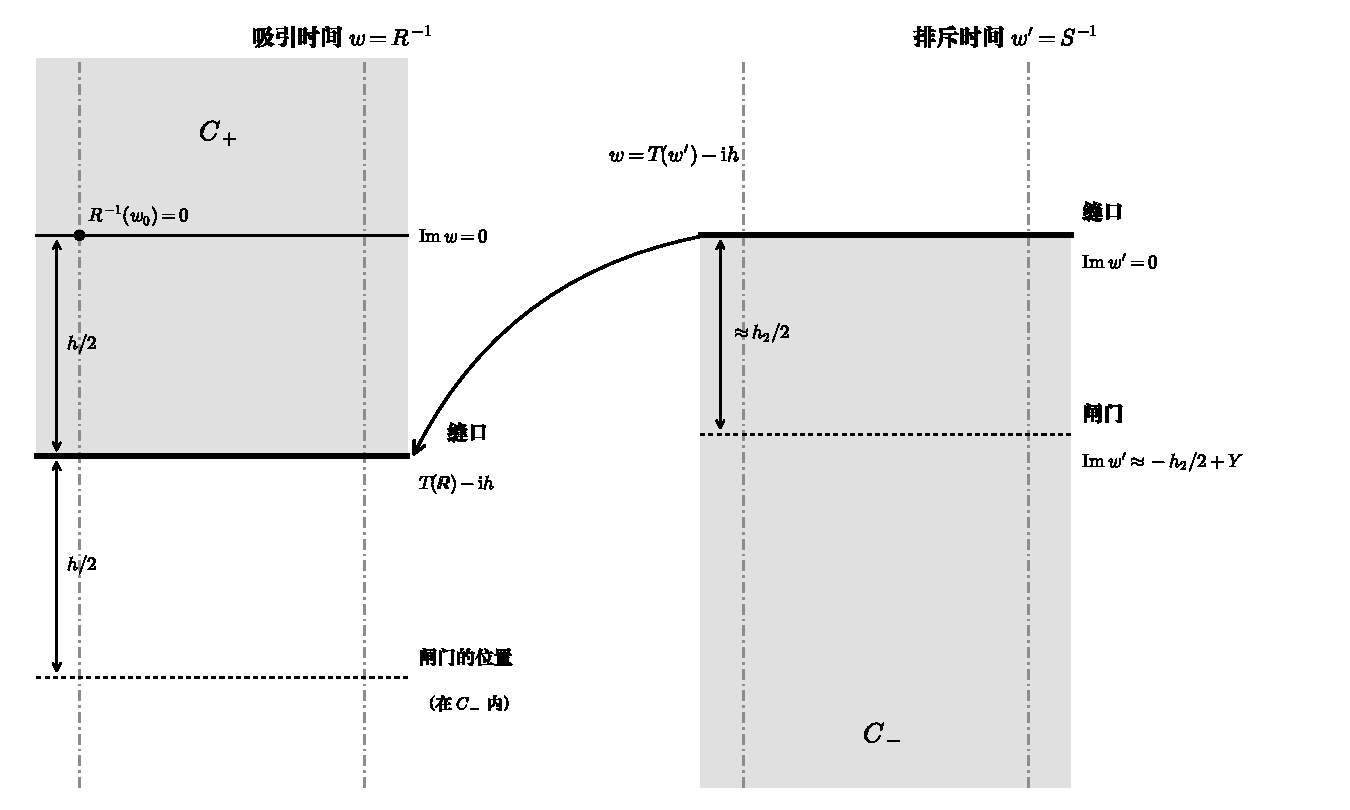
\includegraphics[width=0.8\textwidth]{figures/fig5_cylinders.pdf}
\caption{缝合的两个半柱面（示意图，不按比例；\texttt{figures/fig5\_cylinders.py}）。左：吸引时间 $w=R^{-1}$，
上半柱面 $C_+=\{\Ima w\ge-h/2\}/\Z$。右：排斥时间 $w'=S^{-1}$，下半柱面 $C_-=\{\Ima w'\le0\}/\Z$。
右侧缝口上的点 $w'$ 粘到左侧的 $T(w')-\ii h$。闸门（第~\ref{ch:confluence} 章中 $T$ 收敛到逆 horn 映射的地方）
在排斥时间里位于缝口下方约 $h_2/2$ 处；换到吸引时间，它在缝口下方约 $h/2$、实轴下方约 $h$ 处。}
\label{ch5:fig:cylinders}
\end{figure}

% ======================================================================
\section[算例]{算例：tetration，$b=1.3$}\label{ch5:sec:example}

\begin{example}\label{ch5:exa:b13}
取 tetration（第~\ref{ch:unfolding} 章的 $u$ 坐标，$a_2=\frac12$，$\rho=\frac13$），$b=1.3$，基点 $w_0=1$。脚本 \texttt{figures/ch05\_transition\_example.py}
调用 \texttt{docs/transition\_map.py}：后者只用两个 Schröder 级数（$L$ 与 $L_2$ 处各 40 项）计算 $R^{-1}$ 与 $S$，
在水平线 $\Ima z=-1$ 上取 $32$ 个点做离散 Fourier 变换（30 位运算）。得到（数值）
\begin{gather*}
 \lambda_1=0.385934936554,\quad \lambda_2=2.06141317173,\quad h=6.59938506301,\\
 \Lam=9.8154483\times10^{-19},\quad p=0.6887315094,\\
 t_0=-5.4493869591344+3.2996925315034\,\ii,\\
 t_1=2.79582973902\times10^{-11}-8.30315822559\times10^{-11}\,\ii .
\end{gather*}
可以核对本章的几个结论：
\begin{itemize}
\item $\Ima t_0-h/2\approx-2\times10^{-27}$（数值误差量级），即 \cref{lem:realT} 的分支条件；$|t_{-1}-\overline{t_1}|\approx2\times10^{-24}$。
\item $|t_1|=8.7612271\times10^{-11}$，而 $|\tau_1|\Lam^{1/2}=0.0884320857\times9.9072944\times10^{-10}$
  $=8.76123\times10^{-11}$（\cref{ch5:cor:size}）。
\item 规范化系数与比值：
  \begin{gather*}
   \tau_1=0.0884320857\,\ee^{1.577579614\,\ii},\qquad
   \tau_2=0.01205500797\,\ee^{-1.566107319\,\ii},\\
   \tau_3=0.001447001346\,\ee^{1.50807325\,\ii},\qquad
   t_2/t_1^2=1.541515038\,\ee^{1.561918759\,\ii}.
  \end{gather*}
  对照抛物极限（第~\ref{ch:confluence} 章）：$|B_1|=0.0890584364$，$\arg(B_1\ee^{2\pi\ii a})=1.5865330757$，
  $|B_2|=0.0124873841$，$|B_3|=0.0015927899$，$B_2/B_1^2=1.5744226855\,\ee^{1.5868794187\,\ii}$。
  在 $p\approx0.69$ 处，$|\tau_1|,|\tau_2|,|\tau_3|$ 与极限 $|B_n|$ 的相对差约为 $0.7\%$、$3.5\%$、$9\%$，与 $O(p)$ 的收敛速率（\cref{thm:first-order}）相容。
\end{itemize}
\emph{换基点.} 改用 $w_0'=0.5$（它满足 (H4)）。脚本给出 $\Delta=R^{-1}(0.5)=-0.65860846751381$（实数），
$t_0-t_0'=-0.65860846751381=\Delta$，$t_n'=t_n$（$n\ne0$），$|\tau_n'|=|\tau_n|$ 到所有显示的位数，并且
$\arg\tau_1'=-2.560579432=\arg\tau_1+2\pi\Delta\pmod{2\pi}$（差 $3\times10^{-24}$），与 \cref{prop:base-point} 一致。
$t_2/t_1^2$ 两者相同。

\emph{预言.} 若接受 \eqref{ch5:eq:chat-tau}（第~\ref{ch:sewing} 章证明），则 $b=1.3$ 处缝合解的第一个分离系数是
$c_1\approx\Lam\tau_1\approx8.68\times10^{-20}\,\ee^{1.5776\,\ii}$。在实轴附近，按 \cref{ch5:prop:first-sep}，
缝合解与正则解 $R$ 的差约为 $|c_1R'(x)(\ee^{2\pi\ii x}-1)|\lesssim2\times10^{-19}|R'(x)|$：
在 $b=1.3$，两种``半次迭代''在实轴上的差别在第 19 位小数。
\end{example}

\begin{remark}[在哪条线上取样]\label{ch5:rem:sampling}
\cref{ch5:cor:size} 有一个实际的推论。在实轴上取样时，$t_3$ 的大小是 $|\tau_3|\Lam^{3/2}\approx1.4\times10^{-30}$，
不高于这次计算的数值底（30 位运算，实轴上的舍入误差约 $10^{-30}$），所以在实轴上算出的 $\tau_3$ 毫无意义（脚本给出 $|\tau_3|\approx3.5$）。
在 $\Ima z=-1$ 上取样，第 $n$ 个正模被放大 $\ee^{2\pi n}$ 倍，$\tau_3$ 就能算准。更一般地，
正模应当在全纯带中尽量靠下的线上读出。第~\ref{ch:confluence} 章的闸门正是带的下边缘附近、$T$ 的正模变成 $O(1)$ 的地方。
\end{remark}

\cite{KneserPaper} 的表 tab:tau 把 $\tau_1$、$t_2/t_1^2$ 与从 Kneser 型解直接外推得到的 $\hat c_1$、$\Xi_2$ 作比较：
在 $b=1.10$ 处，$\hat c_1$ 与 $\tau_1$ 的模与辐角都一致到 8 位（数值）。这是 \eqref{ch5:eq:chat-tau} 的数值印证。

\begin{example}[其他族；换基点的数值检验]\label{ch5:exa:families}
\cite{KneserPaper} 的一般化检验（\texttt{docs/generality-check-zh.md} §2，脚本 \texttt{docs/generality\_check.py}，60 位运算）
对第~\ref{ch:unfolding} 章的四个族在 $\lambda_1=0.97$ 处计算了转移映射。下面的数都是数值。
\begin{itemize}
\item 分支条件：四个族的 $|\Ima t_0-h/2|$ 分别不超过 $5\times10^{-57}$、$10^{-43}$、$3\times10^{-31}$、$3\times10^{-59}$，与 \cref{lem:realT} 一致。
\item $|\tau_1|/|B_1|-1$ 分别为 $-9.4\times10^{-6}$、$-1.4\times10^{-5}$、$-1.3\times10^{-5}$、$+1.0\times10^{-3}$；
  $p\approx9\times10^{-4}$，所以偏差是 $O(p)$ 的量级。
\item 二次族取三个基点 $w_0=0$、$0.2$、$0.35$：$|\tau_1|/|B_1|$ 三者都等于 $0.999986451728$，
  而一阶系数 $\log(\tau_1/B_1\ee^{2\pi\ii a})/p$ 的实部三者都等于 $-0.01504809108$（十位一致），虚部分别为 $-0.0748$、$7.788$、$115.8$。
  这正是 \cref{prop:base-point}：模长与实部是不变量，辐角与虚部是基点规范。
\end{itemize}
\end{example}

% ======================================================================
\notes

\textbf{来源.} 本章对应 \cite{KneserPaper} 的 The separation is a transition-map invariant 一节：
\cref{ch5:lem:RS}(3) 与 \cref{lem:realT} 对应 Lemma realT 及其前的定义，\cref{ch5:rem:normalisations} 对应式 (taun) 后的讨论，
\cref{thm:welding} 与 \cref{ch5:cor:cn} 对应 Theorem welding 与 Corollary cn，\cref{ch5:prop:gauge} 对应 Remark invariance。
一般开折的版本（基点条件改为 (H4)）见论文 General real saddle-node unfoldings 一节的改写清单。
\cref{prop:base-point} 与 \cref{cor:invariance} 对应该节的 命题~9.6 与推论~9.7；
这里补全了论文中只写了一句话的共轭不变性证明（Koenigs 坐标的变换、$S$ 的平移、借助辅助基点 $w_0'$）。
\cref{lem:realT}(3) 中的 $T'>0$ 在论文中出现于 Proposition weld-parameter 的证明。
\cref{ch5:lem:strip}(2) 的周期性证明（用实轴上辐角为常数排除 $2\pi\ii k$）是本书补的。

\textbf{双坐标.} 用两个不动点处的 Koenigs 坐标描述一个超越函数的``分数次迭代''，在 tetration 的数值文献中早已出现：
Kouznetsov--Trappmann 在 $b=\sqrt2$ 处比较了四个正则超指数 \cite{KouznetsovTrappmann2010}；
Nixon 用 $F=R\circ(\id+\theta)$ 的形式比较非正则解与正则解 \cite{Nixon2022}，
这正是本章 $K=R\circ(\id+P)$ 的写法。本章的新意在于把两个坐标之间的转移映射 $T$ 作为基本对象，
并证明分离系数是它的函数（焊接恒等式）。

\textbf{与开折模的关系.} 当 $s\to0$ 时，$T$ 收敛到逆 horn 映射（第~\ref{ch:confluence} 章），后者是 Écalle--Voronin 模
\cite{Ecalle1981,Voronin1981}。对固定的 $s>0$，$T$ 是两个双曲不动点的 Koenigs 坐标之间的``Glutsyuk 型''转移映射，
它与 Marde\v{s}i\'c--Roussarie--Rousseau 的开折模 \cite{MRR2004} 的确切关系没有推导。
\cref{cor:invariance} 只说明 $|\tau_n|$ 与 $\Rea\kappa^{(n)}_j$ 是不变量；它们是否构成完全不变量，是开放的。

% ======================================================================
\exercises

\begin{exercise}\label{ch5:ex:period}
证明 $R^{-1}$ 的分支相差 $\ii h\Z$，$S^{-1}$ 的分支相差 $\ii h_2\Z$（在 $\sigma_{\rm rep}$ 的值域内）。
由此说明为什么不存在一个同时等于 $R$ 与 $S$ 的平移的解。
\end{exercise}

\begin{exercise}\label{ch5:ex:mobius}
补全 \cref{ch5:exa:mobius} 的细节：验证 $\sigma$、$\sigma_{\rm rep}$ 的公式与 $\lambda_1\lambda_2=1$，并证明 $S(z)=R(z+t_0)$。
若把基点取在 $(L,L_2)$ 中，$\Ima t_0$ 等于什么？这说明 (H4) 中``基点在 $L$ 远侧''的作用。
\end{exercise}

\begin{exercise}\label{ch5:ex:translations}
直接验证 \cref{ch5:rem:normalisations} 中的三条变换规则，并说明：若 $S$ 换成 $\sigma_{\rm rep}^{-1}(-c\lambda_2^z)$（$c>0$），
则 $\tau_n$ 不变。若 $c<0$ 呢？
\end{exercise}

\begin{exercise}\label{ch5:ex:conj}
设 $s$ 为实数。证明 $\overline{T(\bar z)}=T(z)-\ii h$（在 $\Ima t_0=h/2$ 的分支上），并由此再证一次 $t_{-n}=\overline{t_n}$。
\end{exercise}

\begin{exercise}\label{ch5:ex:real-K}
设 $K$ 是双侧解，实轴含于 $U_+$，并且 $K$ 在实轴上取实值。证明 $P$ 是常数，从而 $K$ 是 $R$ 的平移。
由此说明：$c_1\ne0$ 的双侧解在实轴上不可能是实值的。
\end{exercise}
\begin{hint}
对实的 $x$，$K(x)$ 在 $\mathcal A(L)$ 中的实点，$\Ima R^{-1}(K(x))\in\frac h2\Z$。所以 $\Ima P$ 在实轴上是常数；
一个只有非负模的周期函数，若虚部在实轴上为常数，则它是常数。
\end{hint}

\begin{exercise}\label{ch5:ex:welding-trivial}
设 $\varphi_-=\id-g_0$（即 $G\equiv g_0$）。证明 \eqref{ch5:eq:welding} 化为 $t_n=c_n\ee^{2\pi\ii ng_0}$，并解释：
此时 $T=\varphi_+\circ(\id+g_0)$ 只有非负模，而由 \cref{lem:realT}(2)，这只能在 $T$ 是平移时发生。
\end{exercise}

\begin{exercise}\label{ch5:ex:negative}
仿照 \cref{thm:welding} 的证明，导出负模的公式 $t_{-n}=[G]_{-n}+\sum_{m\ge0}c_m[\ee^{2\pi\ii mG}]_{-n-m}$（$n\ge1$）。
\end{exercise}

\begin{exercise}\label{ch5:ex:first-two}
写出 \eqref{ch5:eq:welding} 在 $n=1,2$ 时的前两项。设 $|c_m|\le C\Lam^m$，并且在 $\Ima w=-Y$ 上 $|G-g_0|\le\epsilon$。
用 $[F]_k$ 在不同高度上计算的自由，估计 $|[\ee^{2\pi\ii mG}]_{-k}|$，并说明在什么条件下 $t_1\ee^{-2\pi\ii g_0}=c_1(1+O(\Lam))$。
\end{exercise}
\begin{hint}
$[F]_{-k}=\int_0^1F(x-\ii Y)\ee^{2\pi\ii k(x-\ii Y)}\dd x$，其模不超过 $\sup|F|\,\ee^{2\pi kY}$；$Y$ 应取得尽量小，即尽量靠近缝口。
\end{hint}

\begin{exercise}\label{ch5:ex:gauge}
设 $K$ 是双侧解，$K(0)=w_0$。对复数 $\delta$，$K(\cdot+\delta)$ 的值 $K(\delta)$ 一般不是实数。说明为什么
$|c_1|$ 的``物理意义''需要基点是实数，并验证 \cref{prop:base-point}(3)。
\end{exercise}

\begin{exercise}\label{ch5:ex:numerics}
运行 \texttt{figures/ch05\_transition\_example.py}，把取样线改为 $\Ima z=0$ 与 $\Ima z=-2$，比较 $\tau_1,\tau_2,\tau_3$。
在 $b=1.3$ 处，$T$ 的全纯带大约有多宽？用 \cref{ch5:cor:size} 解释你看到的现象。
\end{exercise}

\begin{exercise}\label{ch5:ex:invariance-quad}
设 $A(w)=\alpha w+\beta$，$\alpha>0$，$\tilde f_s=A\circ f_s\circ A^{-1}$，$\tilde w_0=A(w_0)$。
不经 \cref{cor:invariance}，直接证明 $\tilde R=A\circ R$、$\tilde S=A\circ S(\cdot-c')$（求出 $c'$），从而 $\tilde\tau_n=\tau_n$（不只是模相等）。
$\alpha<0$ 时会发生什么？
\end{exercise}
\begin{hint}
$\alpha<0$ 时 $a_2$ 变号，需要先用 第~\ref{ch:unfolding} 章的符号约定翻转；上下半平面互换，逆上 horn 映射换成逆下 horn 映射。
\end{hint}
